% !TeX spellcheck = en
\documentclass{article}
\usepackage[utf8]{inputenc}
\usepackage{graphicx}
\usepackage{hyperref}
\usepackage{tikz}
\usepackage{float}
\usepackage[simplified]{pgf-umlcd}
\usetikzlibrary{positioning,fit,calc,arrows.meta, shapes}
\graphicspath{ {images/} }

%Tot això hauria d'anar en un pkg, però no sé com és fa
\newcommand*{\assignatura}[1]{\gdef\1assignatura{#1}}
\newcommand*{\grup}[1]{\gdef\3grup{#1}}
\newcommand*{\professorat}[1]{\gdef\4professorat{#1}}
\renewcommand{\title}[1]{\gdef\5title{#1}}
\renewcommand{\author}[1]{\gdef\6author{#1}}
\renewcommand{\date}[1]{\gdef\7date{#1}}
\renewcommand{\maketitle}{ %fa el maketitle de nou
    \begin{titlepage}
        \raggedright{UNIVERSITAT DE LLEIDA \\
            Escola Politècnica Superior \\
            Grau en Enginyeria Informàtica\\
            \1assignatura\\}
            \vspace{5cm}
            \centering\huge{\5title \\}
            \vspace{3cm}
            \large{\6author} \\
            \normalsize{\3grup}
            \vfill
            Professorat : \4professorat \\
            Data : \7date
\end{titlepage}}
%Emplenar a partir d'aquí per a fer el títol : no se com es fa el package
%S'han de renombrar totes, inclús date, si un camp es deixa en blanc no apareix

\tikzset{
	%Style of nodes. Si poses aquí un estil es pot reutilitzar més facilment
	pag/.style = {circle, draw=black,
                           minimum width=0.75cm, font=\ttfamily,
                           text centered}
}
\title{WebProject: Pre-assignment}
\author{Pau Ibáñez Millán, Joan Martí Olivart, Ian Palacín Aliana, Joaquim Picó Mora, Sergi Simón Balcells}
\date{Diumenge 12 de Gener}
\assignatura{Web Project}
\professorat{F. Verdés}
\grup{PraLab1}

%Comença el document
\begin{document}
	\maketitle
	\thispagestyle{empty}
	
	\newpage
	\pagenumbering{roman}
	\tableofcontents
	\newpage
	\pagenumbering{arabic}
	
\section{Our Idea}
\section{API's}
\section{Model}
 \begin{figure}[h]
 	\centering
 	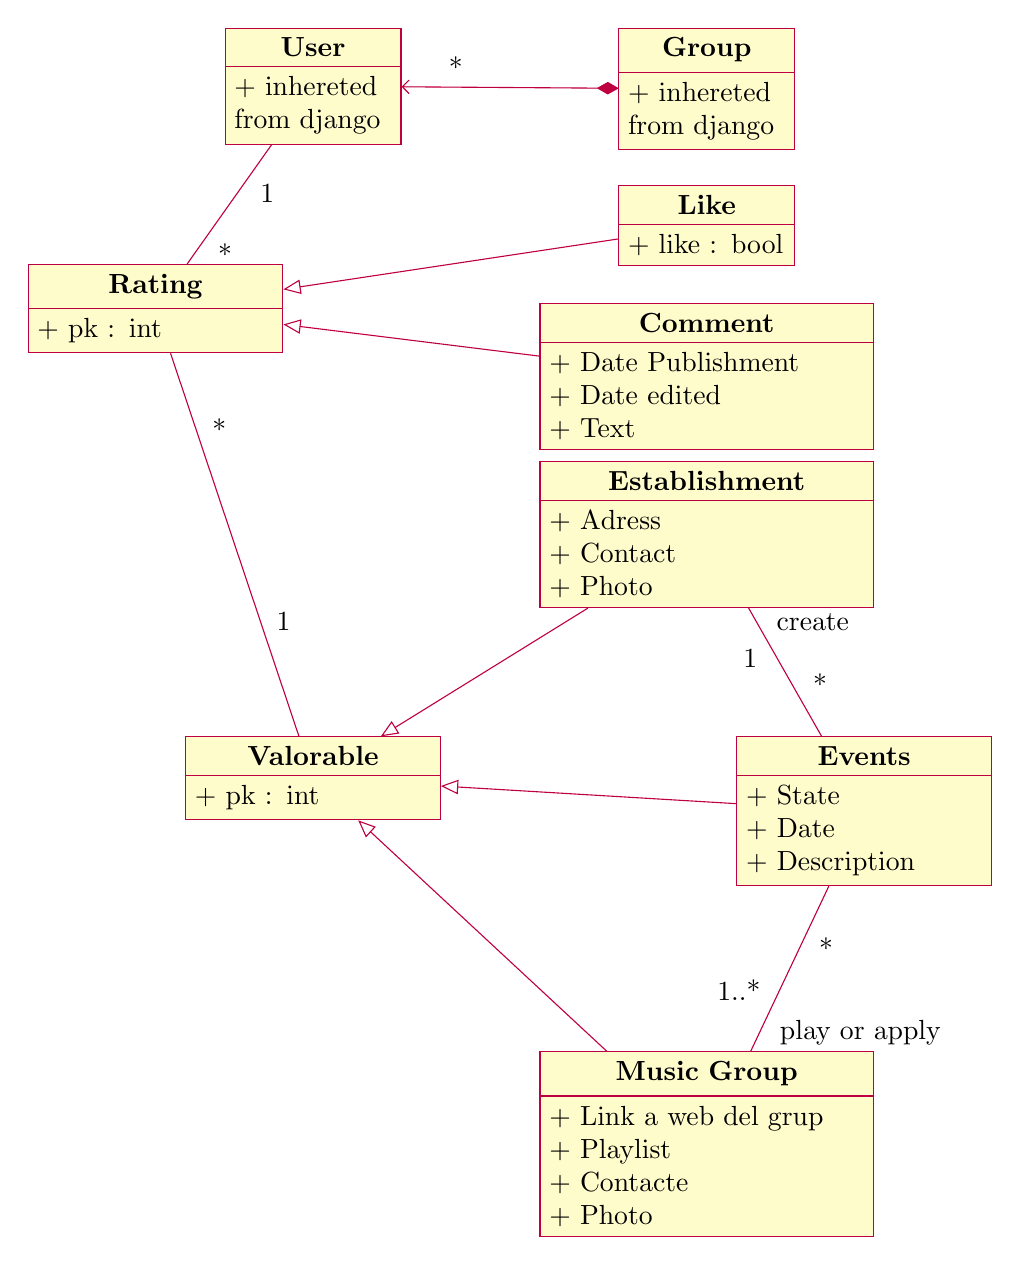
\begin{tikzpicture}
 	\begin{class} [text width=3cm]{Valorable}{0, -9}
	\attribute{+ pk : int} 	

 	
 	\end{class}
 	\begin{class} [text width=4cm]{Music Group}{5, -13}
 	\inherit{Valorable}	
 	 	\attribute{+ Link a web del grup}
 	\attribute{+ Playlist}
 	\attribute{+ Contacte}
 	\attribute{+ Photo}

 	
 	\end{class}
 	\begin{class} [text width=4cm]{Establishment}{5, -5.5}
 	\inherit{Valorable}	
 	
 	
 	\attribute{+ Adress}
 	\attribute{+ Contact}
 	\attribute{+ Photo}
 	
 	\end{class}
 	\begin{class} [text width=3cm]{Events}{7, -9}
 	\inherit{Valorable}	
 	
 	\attribute{+ State }
 	\attribute{+ Date}
 	\attribute{+ Description}
 	
 	\end{class}
 	
 	\begin{class} [text width=3cm]{Rating}{-2, -3}
 	\attribute{+ pk : int} 	
 	
 	
 	\end{class}
 	\begin{class} [text width=4cm]{Comment}{5, -3.5}
 	\inherit{Rating}	
 	\attribute{+ Date Publishment }
 	\attribute{+ Date edited}
 	\attribute{+ Text}
 	
 	
 	\end{class}
 	\begin{class} [text width=2cm]{Like}{5, -2}
 	\inherit{Rating}
 	
 	
 	\attribute{+ like : bool}
 	
 	\end{class}
 	\begin{class} [text width=2cm]{User}{0,0}
 	
 	\attribute{+ inhereted from django}
 	
 	\end{class}
 	\begin{class} [text width=2cm]{Group}{5, 0}
 	
 	
 	\attribute{+ inhereted from django}
 	
 	\end{class}
 	
 	% Assotiations
 	\association{User}{1}{}{Rating}{*}{}
 	\composition{Group}{}{*}{User}
 	\association{Rating}{*}{}{Valorable}{1}{}
 	\association{Events}{*}{}{Music Group}{play or apply}{1..*}
 	\association{Events}{}{*}{Establishment}{1}{create}
 	\end{tikzpicture}
 	\caption{Model}
 \end{figure}
\end{document}






















